% !TEX root = perelman-geometry.tex
%!TEX TS-program = pdflatex
%!TEX encoding = UTF-8 Unicode

\setchapterpreamble[o]{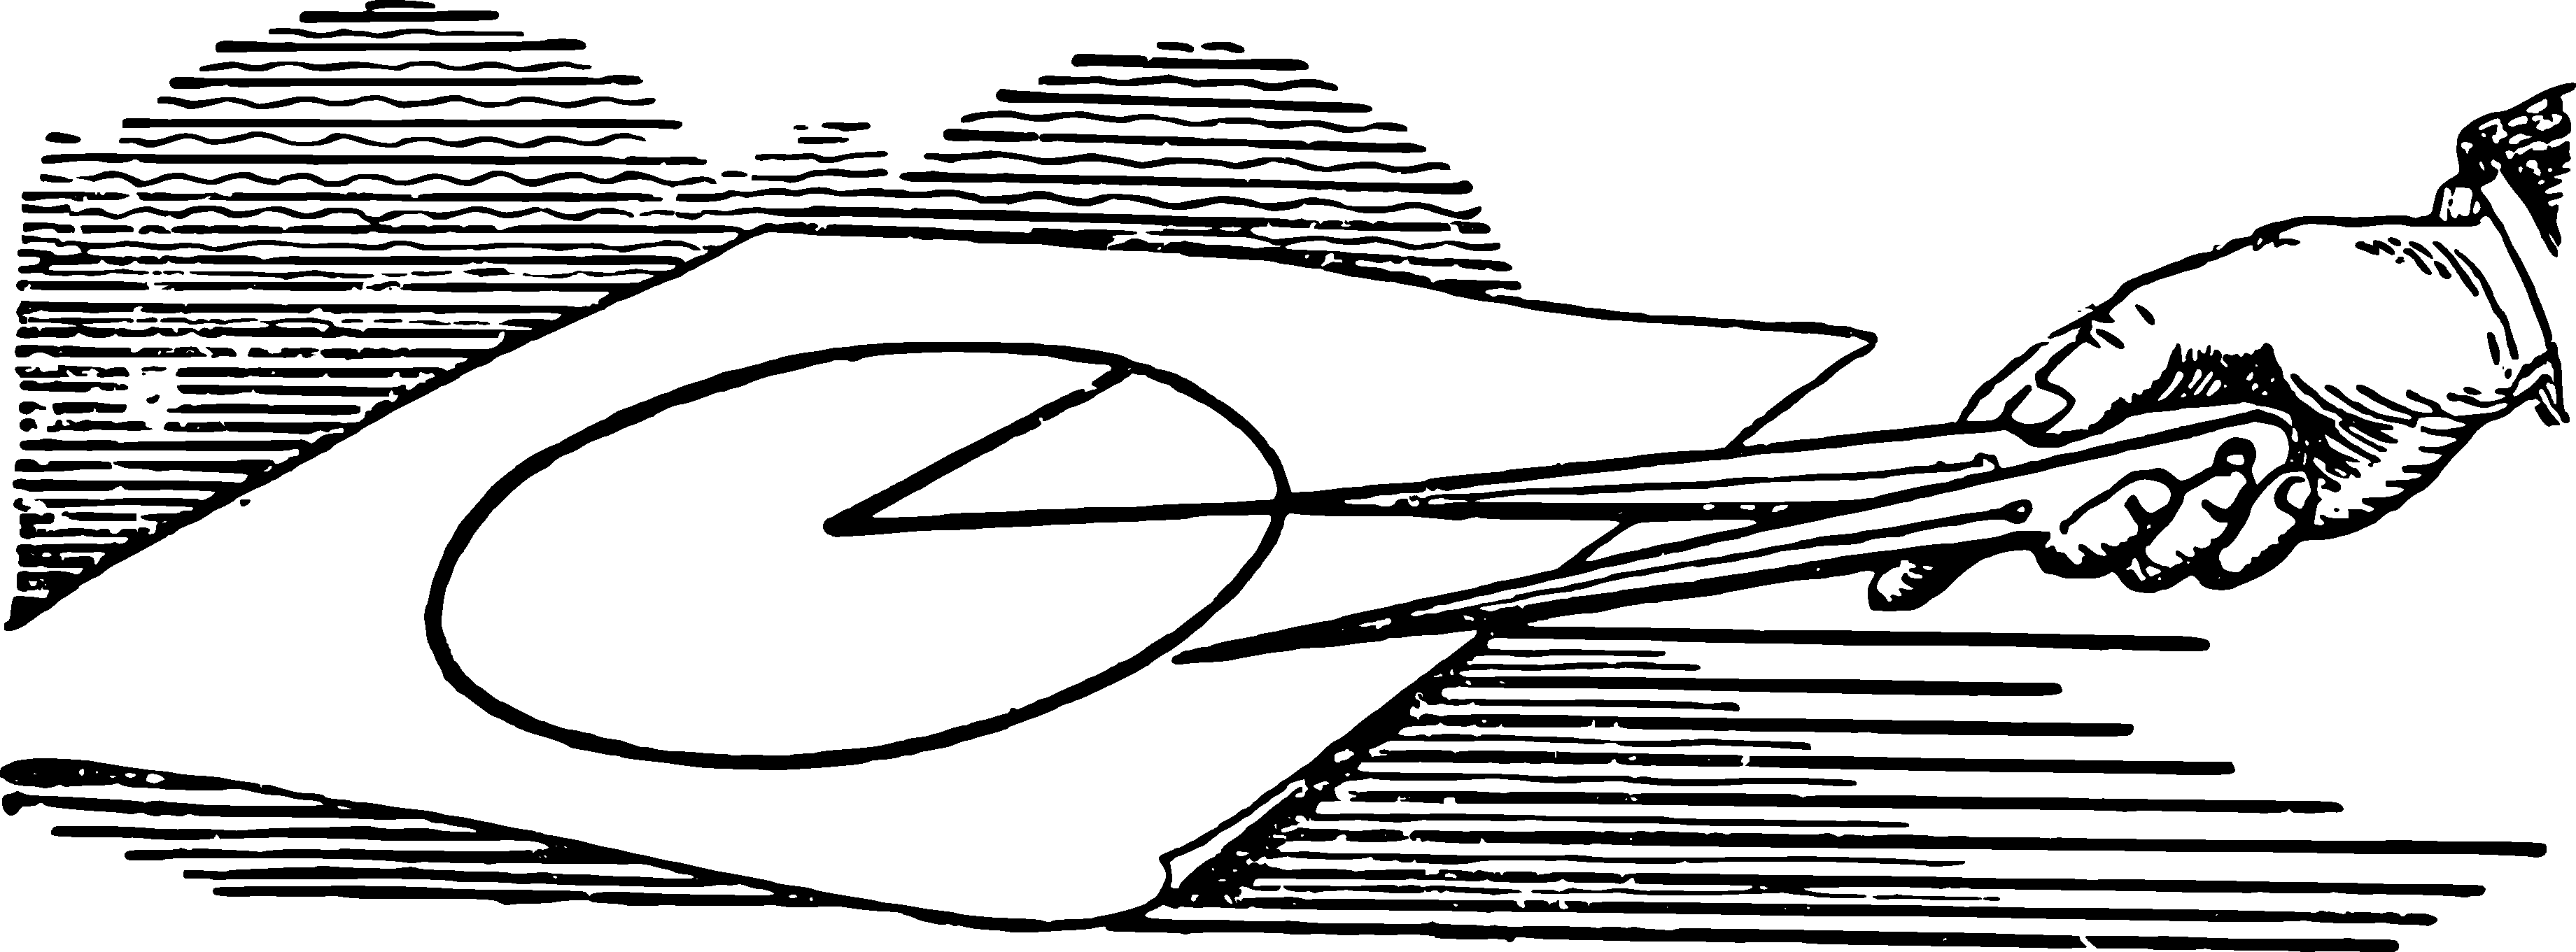
\includegraphics[width=1.2\textwidth]{figures/ch-05/fig-ch-05-head.pdf}\bigskip}

\chapter{Field Trigonometry Without Formulas and Tables}
\label{ch-05}
	
\section{Calculation of the sine}
\label{sec-5.1}

In this chapter, we will demonstrate how to calculate the sides of a triangle with an accuracy of 2\% and angles with an accuracy of \ang{1}, using only the concept of sine and without resorting to tables or formulas. Such simplified trigonometry can be useful during outdoor walks when tables are not at hand, and formulas are half-forgotten. Robinson Crusoe on his island could successfully employ such trigonometry.
\begin{marginfigure}%t[h!]
\centering
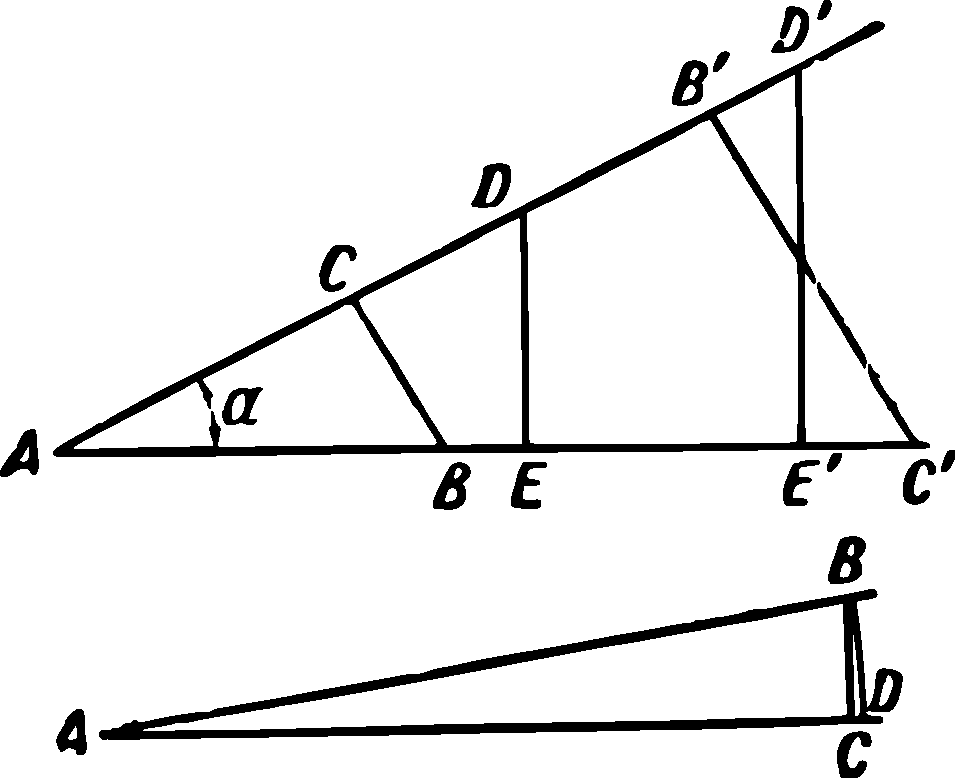
\includegraphics[width=\textwidth]{figures/ch-05/fig-088.pdf}
\sidecaption{What is the sine of an acute angle?\label{fig-088}}
\end{marginfigure}

So, imagine that you have not yet studied trigonometry or have forgotten it entirely -- a state that some readers may easily imagine. Let's begin to acquaint ourselves with it again. What is the sine of an acute angle? It is the ratio of the opposite side to the hypotenuse in the triangle formed by dropping a perpendicular from the angle to one of its sides. For example, the sine of angle $a$ (\figr{fig-088}) is $BC/AB$, or $ED/AD$, or $D'E'/AD'$, or $B'C'/AC'$. It is easy to see that due to the similarity of the triangles formed here, all these ratios are equal to each other.

Let's find the sine values of various angles from \ang{1} to \ang{90}. How can we do this without having tables at hand? Quite simply: we need to create our own table of sines. That's exactly what we'll do now.

Let's start with angles whose sine values we know from geometry. Firstly, the angle of \ang{90}, whose sine is obviously 1. Then the angle of \ang{45}, the sine of which can be easily calculated using the Pythagorean theorem; it equals $\sqrt{2}/2$, which is approximately 0.707. Next, we know the sine of \ang{30}; since the side opposite such an angle is half the hypotenuse, the sine of $\ang{30} = 1/2$.

So, we know the sines (or, as commonly denoted, sin) of three angles: 
\begin{align*}%
\sin \ang{30} & = 0.5, \\
\sin \ang{45} & = 0.707, \qand \\
\sin \ang{90} & = 1.
\end{align*}
Of course, this is not enough; we need to know the sines of all intermediate angles at least through every degree. For very small angles, we can approximate the sine by taking the ratio of the arc to the radius without much error: from \figr{fig-088} (lower),
shows that the ratio $\overline{BC}/AB$ differs little from the $\ \wideparen{BD}/AB$ ratio. For example, for an angle of \ang{1}, the arc $BD = 2\pi R/360$ and, therefore, $\sin \ang{1}$ can be taken equal to
\begin{equation*}%
\frac{2 \pi R}{360 , R} = \frac{\pi}{180} = 0.0175. 
\end{equation*}
Using the same method, we find: 
\begin{align*}%
\sin \ang{2} & = 0.0349, \\
\sin \ang{3} & = 0.0524,\\
\sin \ang{4} & = 0.0698, \\
\sin \ang{5} & = 0.0873.
\end{align*}
However, we need to determine how far we can extend this table without introducing significant errors. If we were to compute sin \ang{30} using this method, we would obtain 0.524 instead of 0.500; the difference would already be in the second significant digit, and the margin of error would be 24/500, i.e. about 5\%.

This is too crude even for basic field trigonometry. To find the limit to which we can calculate sine values using the approximate method described, let's try to find $\sin \ang{15}$ using a more precise method. To do this, we'll employ the following relatively straightforward construction (\figr{fig-89}).

\begin{marginfigure}%t[h!]
\centering
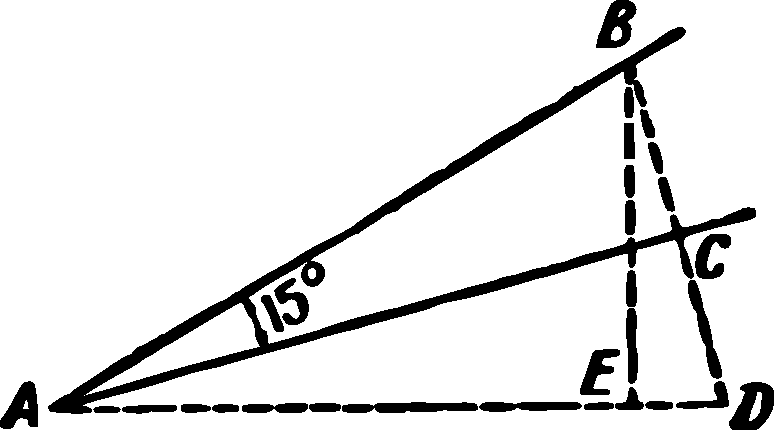
\includegraphics[width=\textwidth]{figures/ch-05/fig-089.pdf}
\sidecaption{How to calculate $\sin \ang{15}$?\label{fig-089}}
\end{marginfigure}

Let $\sin \ang{15} = BC/AB$. Let us extend $BC$ by an equal distance to the point $D$; connect $A$ with $D$, then we get two equal triangles: $ADC$ and $ABC$, with the angle $BAE$ equal to \ang{30} degrees. We'll drop a perpendicular $BE$ on $AD$ from point $B$, creating a right triangle $BAE$ with a \ang{30} angle $(< BAE)$, then $BE = AB/2$. Next, we'll calculate $AE$ using the Pythagorean theorem in triangle $ABE$:
\begin{align*}%
AE^{2} & = AB^{2} - \left(\frac{AB}{2} \right)^{2}= \frac{3}{4}\, AB^{2},\\
AE & = \frac{AB}{2} \sqrt{3} = 0.866 \, AB.
\end{align*}
Thus, $ED = AD - AE = AB - 0.866 AB = 0.134 AB$. Now, from triangle $BED$, we'll calculate $BD$:
\begin{align*}%
BD^{2} & = BE^{2} + ED^{2} = \left(\frac{AB}{2} \right)^{2} + (0.134AB)^{2} = 0.268\, AB^{2}\\
BD & = \sqrt{0.268AB^{2}} = 0.518 \, AB.
\end{align*}
Half of $BD$, i.e., $BC$, equals $0.259\, AB$, therefore the sine of angle $BAD$ is the same as the sine of \ang{15}.
\begin{equation*}%
\sin \ang{15} = \frac{BC}{AB} = \frac{0.259 \,AB}{AB} = 0.259.
\end{equation*}
This is the tabular value of $\sin \ang{15}$ if we limit ourselves to three significant figures. The approximate value we would have found using the previous method is 0.262. Comparing the values 0.259 and 0.262, we see that by rounding to two significant figures, we obtain 0.26 and 0.26, which are identical results. The error in replacing the more accurate value (0.259) with the approximate one (0.26) is 1/1000 times the difference, i.e., about 0.4\%. This margin of error is acceptable for field calculations, so we are justified in calculating the sines of angles from 1 to 15 degrees using our approximate method.

For the range from \ang{15} to \ang{30} degrees, we can compute the sines using proportions. We reason as follows: the difference between $\sin \ang{30}$ and $\sin \ang{15}$ is $0.50 - 0.26 = 0.24$. Therefore, we can assume that for each degree increase, the sine increases by approximately 1/15 of this difference, i.e., $0.24/15 = 0.016$. Strictly speaking, this is not precisely accurate, but the deviation from the rule only becomes apparent in the third significant digit, which we discard anyway. Thus, by adding 0.016 successively to $\sin \ang{15}$, we get the sines of \ang{16}, \ang{17}, \ang{18}, etc.:
%\begin{center}
%\begin{tabular}{c}%
%\toprule
%$\sin \ang{16} = 0.26 + 0.016 = 0.28$,\\
%$\sin \ang{17} = 0.26 + 0.032 = 0.29$,\\
%$\sin \ang{18} = 0.26 + 0.048 = 0.31$,\\
%$\sin \ang{25} = 0.26 + 0.16 = 0.42$,\\
%and so on.\\
%\bottomrule
%\end{tabular}
%\end{center}
\begin{small}
\begin{align*}%
\sin \ang{16} &= 0.26 + 0.016 = 0.28,\\
\sin \ang{17} &= 0.26 + 0.032 = 0.29,\\
\sin \ang{18} &= 0.26 + 0.048 = 0.31,\\
\sin \ang{25} &= 0.26 + 0.16 = 0.42,\,\,\text{and so on.}
\end{align*}\label{page-130}
\end{small}
All these sines are accurate to the first two decimal places, which is sufficient for our purposes; they differ from the true sines by less than half the value of the last digit.

Using the same method, we calculate angles within the range between \ang{30} and \ang{45} degrees. The difference between $\sin \ang{45} - \sin \ang{30} = 0.707 - 0.5 = 0.207$. Dividing this difference by 15, we get 0.014. We'll add this value successively to $\sin \ang{30}$, resulting in:
%\begin{center}
%\begin{tabular}{c}%
%\toprule
%$\sin \ang{31} = 0.5 + 0.014 = 0.51$,\\
%$\sin \ang{32} = 0.5 + 0.028 = 0.52$,\\
%\ldots \quad \ldots \\
%$\sin \ang{40} = 0.5 + 0.014 = 0.64$,\\
%and so on.\\
%\bottomrule
%\end{tabular}
%\end{center}
\begin{small}
\begin{align*}%
\sin \ang{31}  & = 0.5 + 0.014 = 0.51,\\
\sin \ang{32}  & = 0.5 + 0.028 = 0.52,\\
\ldots & \ldots \\
\sin \ang{40}  & = 0.5 + 0.014 = 0.64,\,\,\text{and so on.}
\end{align*}
\end{small}
\begin{marginfigure}[2cm]
\centering
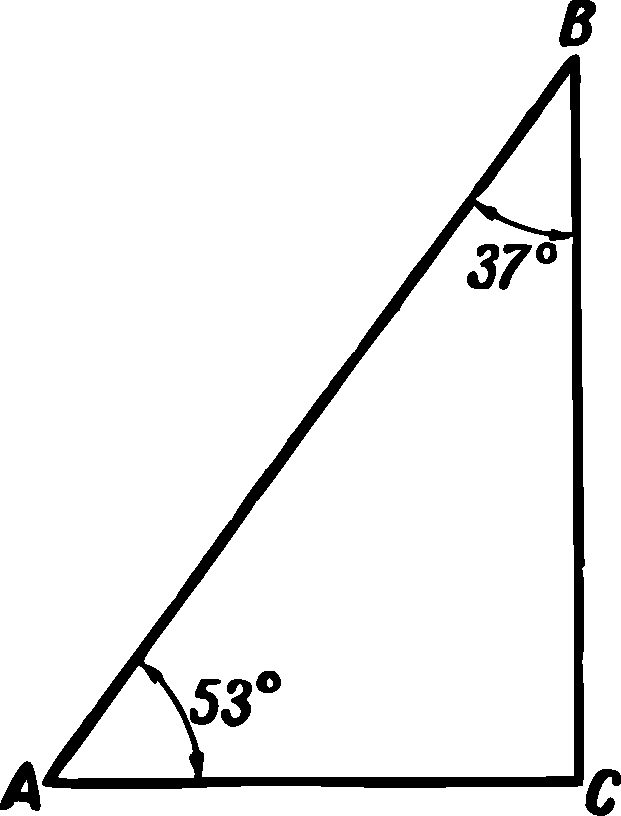
\includegraphics[width=0.8\textwidth]{figures/ch-05/fig-090.pdf}
\sidecaption{To calculate the sine of an angle greater than \ang{45}.\label{fig-090}}
\end{marginfigure}
We also need to find the sines of acute angles larger than \ang{45}. The Pythagorean theorem can help us with this. Let's say we want to find $\sin \ang{53}$ (\figr{fig-90}), which corresponds to the ratio of side $BC/AB$. Since angle $B = \ang{37}$, we can compute its sine using the method described earlier: it equals $0.5 + 7 \times 0.014 = 0.6$. On the other hand, since we know that $\sin B = AC/ AB$, so $AC/AB = 0.6$ or $AC = 0.6 \, AB$. Knowing $AC$, we can easily calculate $AC$. This segment equals $\sqrt{(AB^{2} - BC^{2})} = \sqrt{(AB^{2} - (0.6AB)^{2})} = 0.8\, AB$. Overall, the calculation is straightforward; we just need to be able to compute square roots.


\section{Extraction of the square root}
\label{sec-5.2}

The method for extracting square roots mentioned in algebra courses is easily forgotten. But one can do without it. In many geometry textbooks, an ancient simplified method for computing square roots using the division method is presented. Here, I will share another old method, which is also more straightforward than the one considered in algebra courses.

Let's say we need to compute the square root of 13. It lies between the square roots of 9 and 16, therefore, it is equal to 3 plus a fraction denoted by $x$.

So,
\begin{align*}%
\sqrt{13} & = 3 + x, \,\, \text{hence} \\
13 & = 9 + 6x + x^{2}.
\end{align*}
Since the square of the fraction $x$ is a small fraction that can be neglected in the first approximation, we have:
\begin{align*}%
13 &= 9 - 6x, \,\, \text{this leads to} \\
6x & = 4,\,\, \text{hence,}
x & = 4/6 = 0.67.
\end{align*}
Therefore, approximately, $\sqrt{13} = 3.67$. If we want to determine the value of the root more precisely, we can write the equation $\sqrt{13} = 3 \, 2/3+ + y$, where $y$ is a small positive or negative fraction. From this equation, we have
\begin{equation*}%
13 = \frac{121}{9}  + \frac{22}{3} y  + y^{2}.
\end{equation*}
Neglecting $y^{2}$, we find that $y$ is approximately equal to $-0.06$. Thus, in the second approximation, $\sqrt{13} = 3.67 - 0.06 = 3.61.$

The third approximation can be found using the same method, and so on. Using the conventional method taught in algebra courses, we would find the square root of 13 accurate to 0.01, also as 3.61.


\section{To find an angle from its sine}
\label{sec-5.3}

So, we have the ability to compute the sine of any angle from \ang{0} to \ang{90} with two decimal places. The need for a ready-made table is eliminated; for approximate calculations, we can always create it ourselves if desired.

But to solve trigonometric problems, one also needs to be able to compute angles from a given sine. This is also not difficult. Let's say we need to find the angle whose sine is 0.38. Since this sine is less than 0.5, the angle we seek is less than \ang{30}. But it is greater than \ang{15}, as the sine of \ang{15}, we know, is 0.26. To find this angle, which lies between \ang{15} and \ang{30}, we proceed as explained on page~\pageref{page-130}:
\begin{align*}%
0.38 - 0.26 & = 0.12,\\
\frac{0.12}{0.016} & = \ang{7.5},\\
\ang{15}  + \ang{7.5} & = \ang{22.5}.
\end{align*}
So, the angle we seek is approximately \ang{22.5}. Another example: find the angle whose sine is 0.62.
\begin{align*}%
0.62 - 0.50 & = 0.12,\\
\frac{0.12}{0.014} & = \ang{8.6},\\
\ang{30}  + \ang{8.6} & = \ang{38.6}.
\end{align*}
The angle we seek is approximately \ang{38.65}.

Finally, the third example: find the angle whose sine is 0.91.

Since this sine lies between 0.71 and 1, the angle we seek lies between \ang{45} and \ang{90}. In \figr{fig-091}, $BC$ is the sine of angle $A$, if $BA = 1$.

\begin{marginfigure}%[2cm]
\centering
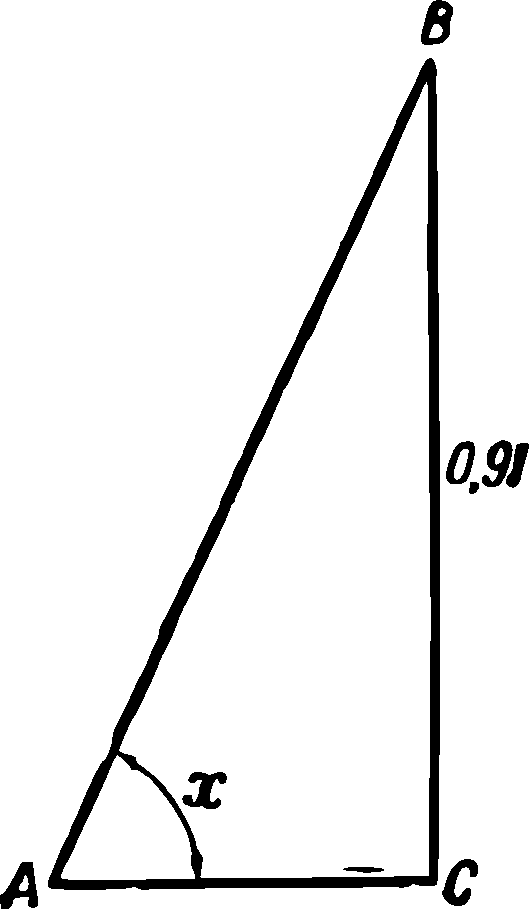
\includegraphics[width=0.8\textwidth]{figures/ch-05/fig-091.pdf}
\sidecaption{To calculate an acute angle by its sine.\label{fig-091}}
\end{marginfigure}

Knowing $BC$, it is easy to find the sine of angle $B$: BC
\begin{align*}%
AC^{2} & = 1 - BC^{2} = 1 - 0.91^{2}\\
AC^{2} &  = 1 - 0.83 = 0.17,\\
AC & = \sqrt{0.17} = 0.42.
\end{align*}
Now let's find the value of angle $B$, whose sine is 0.42; after that, it will be easy to find angle $A$, which is equal to $\ang{90}  - B$. Since 0.42 lies between 0.26 and 0.5, angle $B$ lies between \ang{15} and \ang{30}. It is determined as follows:
\begin{align*}
0.42 - 0.26 & = 0.16, \\
\frac{0.16}{0.016} & = \ang{10},\\
B & = \ang{15} + \ang{10} = \ang{25}.
\end{align*}
And that means the angle $A = \ang{90} - B = \ang{90} - \ang{25} = \ang{65}.$

We are now well-equipped to approximately solve trigonometric problems, as we can find sines from angles and angles from sines with an accuracy sufficient for outdoor purposes.

But is the sine alone sufficient for this? Will we not need the other trigonometric functions -- cosine, tangent, etc.? We will now demonstrate with several examples that for our simplified trigonometry, one can easily manage with just the sine.

\section{Height of the Sun Problem}
\label{sec-5.4}

\begin{figure}%[2cm]
\centering
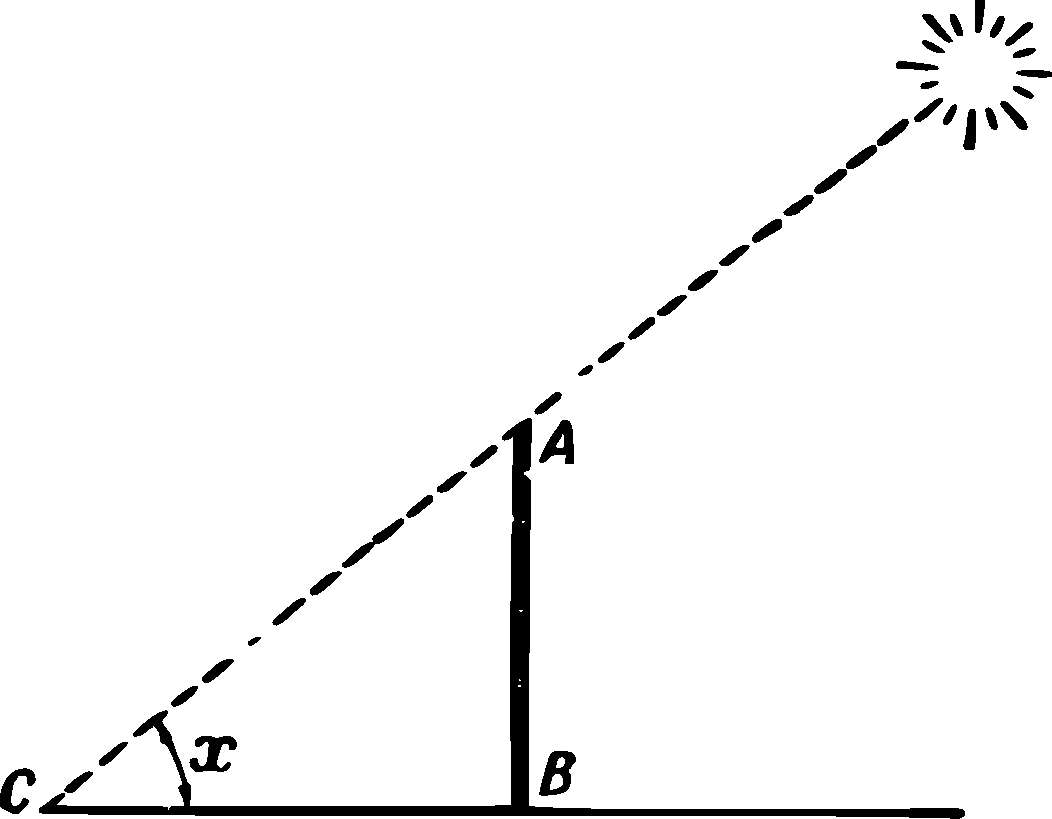
\includegraphics[width=0.7\textwidth]{figures/ch-05/fig-092.pdf}
\sidecaption{To determine the height of the Sun above the horizon.\label{fig-092}}
\end{figure}

\ques The shadow $BC$ (\figr{fig-092}) of the vertical pole $AB$, with a height of 4.2 m, measures 6.5 m. What is the height of the Sun above the horizon, i.e., what is the angle $C$?


\ans It is easy to see that the sine of angle $C$ is equal to $AB/AC$. Since 
\begin{align*}%
AC & = \sqrt{AB^{2} + BC^{2}},\\
& = \sqrt{4.2^{2} + 6.5^{2}},\\ 
& = 7.74. 
\end{align*}
Therefore, the sine we are seeking is approximately $4.2/7.74 = 0.55$. Using the method described earlier, we find the corresponding angle: \ang{33}. The height of the Sun is approximately \ang{33} with an accuracy of \ang{0.5}.

\section{Distance to the Island Problem}
\label{sec-5.5}

While wandering with a compass near the river, you noticed an island $A$ on it (\figr{fig-093}) and wish to determine its distance from point $B$ on the shore. To do this, you determine the angle $ABN$, formed with the north-south direction $(NS)$, by the straight line $BA$ using the compass. Then, you measure the straight line $BC$ and determine the angle $NBC$ between it and $NS$. Finally, you do the same at point $C$ for the straight line $AC$. Let's assume that you obtained the following data:

The direction $AB$ deviates from $NS$ to the east by \ang{52}.
The direction $BC$ deviates from $NS$ to the east by \ang{110}.
The direction $CA$ deviates from $NS$ to the east by \ang{27}.


The length of $BC$ is 137 m. How can you calculate the distance $BA$ using this data?

\begin{figure}[h!]
\centering
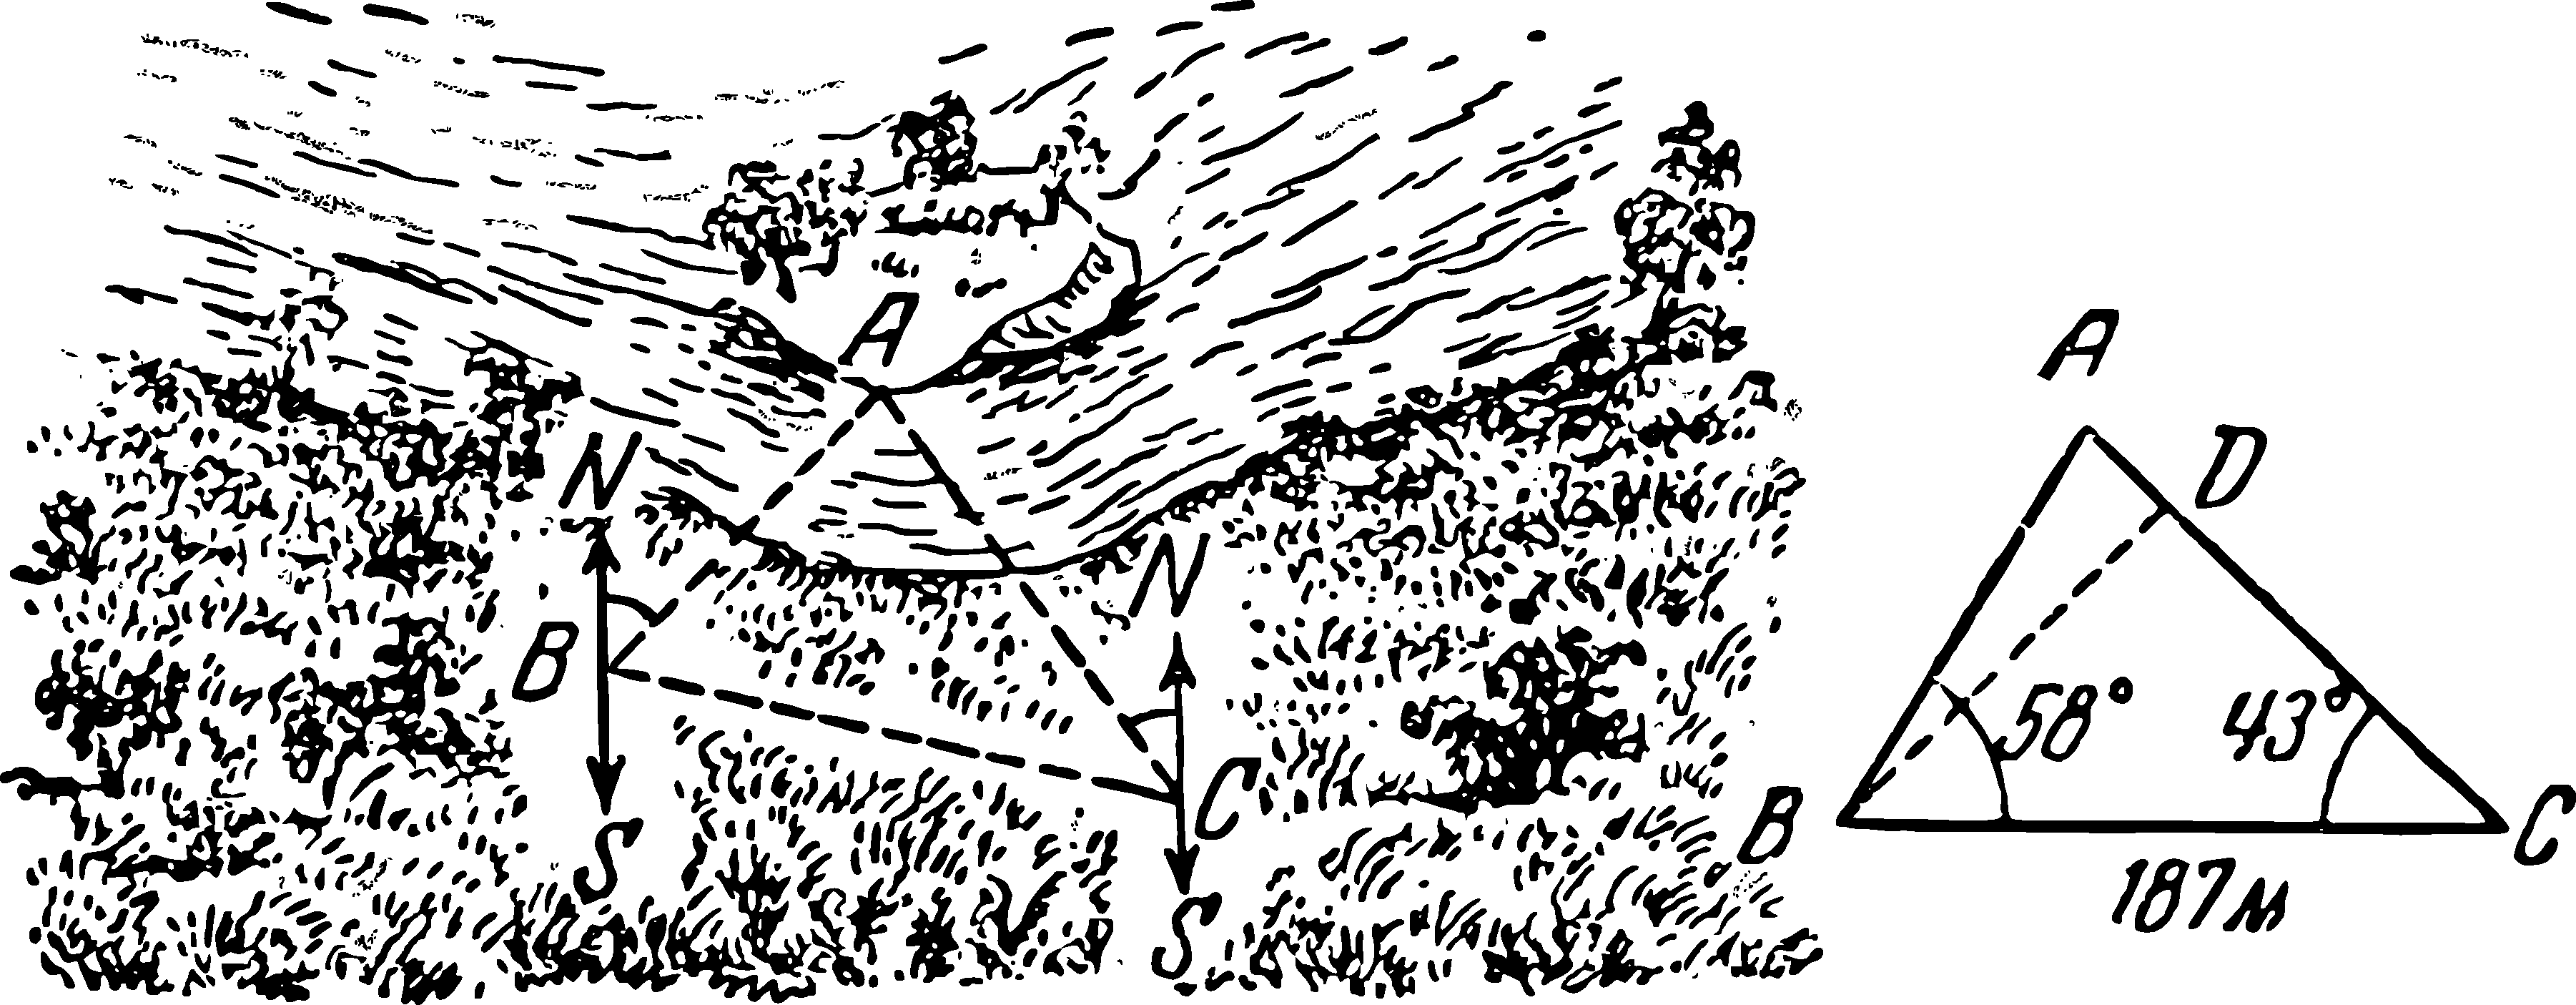
\includegraphics[width=\textwidth]{figures/ch-05/fig-093.pdf}
\sidecaption{How to calculate the distance to the island?\label{fig-093}}
\end{figure}

\ans In triangle $ABC$, we know the side $BC$. Angle $ABC = \ang{110} - \ang{52} = \ang{58}$; angle $ACB = \ang{180} − \ang{110} − \ang{27} = -\ang{43}$. Let's consider the height $BD$ in this triangle (\figr{fig-098}, to the right): $\sin C = \sin \ang{43} = BD/187$. By calculating the $\sin \ang{43}$ using the method mentioned earlier, we obtain approximately 0.68. Hence, 
\begin{equation*}%
BD = 187 \times 0.68 = 127.
\end{equation*}
Now, in triangle $ABD$, we know the side $BD$; angle $A = \ang{180} − (\ang{58} + \ang{43}) = \ang{79}$, and angle $ABD = \ang{90} − \ang{79} = \ang{11}$. We can calculate the $\sin \ang{11}$: it is 0.19. Therefore, $AD/AB = 0.19$. Using the Pythagorean theorem, 
\begin{equation*}%
AB^{2} = BD^{2} + AD^{2}.
\end{equation*}
Substituting $0.19 \, AB$ for $AD$ and 127 for $BD$, we have: 
\begin{equation*}%
AB^{2} = 127^{2} + (0.19AB)^{2}.
\end{equation*}
from which $AB \approx 128$. Thus, the distance to the island is approximately \SI{128}{\meter}. The reader, I believe, would not have difficulty in calculating the direction $AC$ if needed.

\section{Lake Width Problem}
\label{sec-5.6}

To determine the width of lake AB (see \figr{fig-094}), you found from the compass that line $AC$ veers westward by \ang{21}, and $BC$ veers eastward by \ang{22}. With $BC = \SI{68}{\meter}$ and $AB = \SI{35}{\meter}$, calculate the width of the lake.

\begin{figure}[h!]
\centering
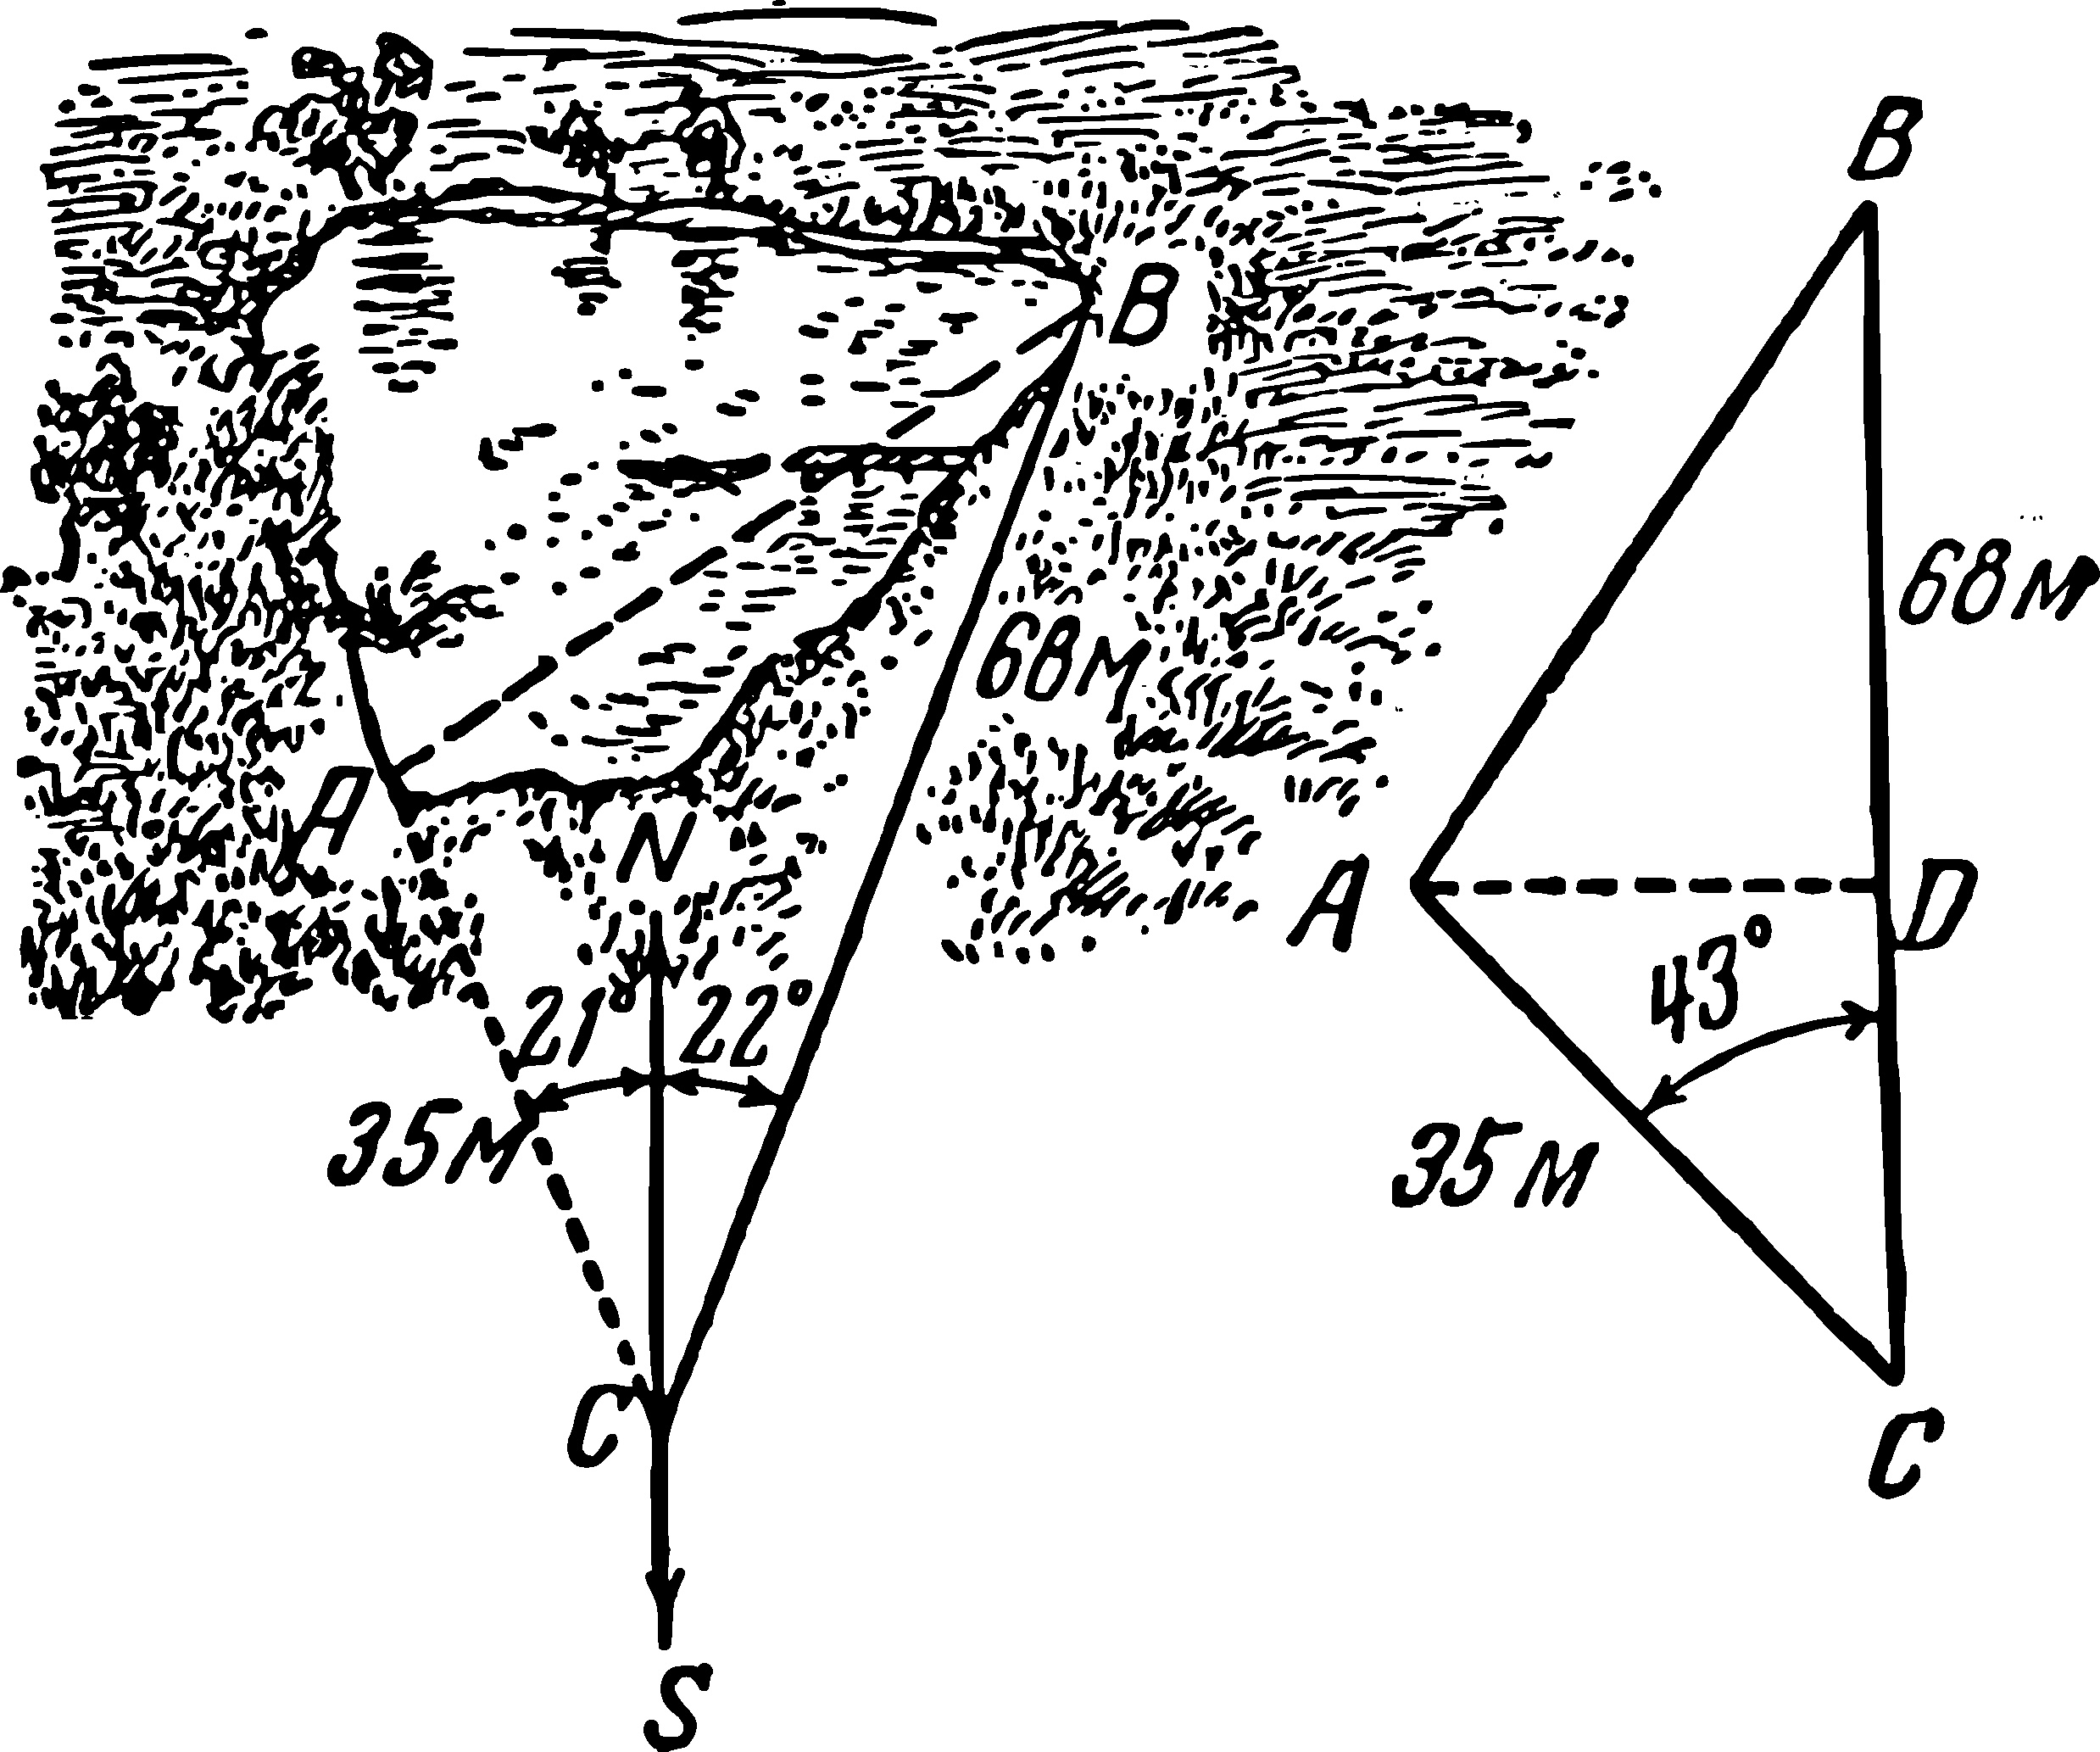
\includegraphics[width=0.8\textwidth]{figures/ch-05/fig-094.pdf}
\sidecaption{How to calculate the width of the lake?\label{fig-094}}
\end{figure}

\ans In triangle $ABC$, we know angle $ABC = \ang{43}$ and the lengths of its sides are \SI{68}{\meter} and \SI{35}{\meter}. Dropping a perpendicular from $A$ to $D$ (to the right), we get a right triangle $ADC$ where the angle $C$ is \ang{43}. Hence $\sin \ang{43} = AD/AC$. Calculating, $\sin \ang{43} = 0.68$, hence $AD = \sin \ang{43} \times AC  = 0.68 \times 35 = 24$. Next, we compute $CD$ and $BD$: 
\begin{align*}%
CD^{2} & = AC^{2} - AD^{2} = 35^{2} - 24^{2} = 649; \therefore CD = 25.5;\\
BD & = BC - CD =  68 - 25.5 = 42.5. 
\end{align*}
Now, from triangle ABD, 
\begin{align*}%
AB^{2} & = AD^{2} + B{D}^2 \\
& = 24^{2} + 42.5^{2} = 2380;\\
AB & \approx 49.
\end{align*}
Thus, the sought width of the lake is about \SI{49}{\meter}.

If we had to calculate the other two angles in triangle $ABC$, having found $AB = 49$, we would proceed as follows: 
\begin{align*}%
\sin B & = \frac{AD}{AB}  = \frac{24}{49} = 0.49,\,\, \text{hence}\\ 
B & = \ang{29}. 
\end{align*}
The third angle $C$ is found by subtracting the sum of angles \ang{29} and \ang{43} from \ang{180}; it equals \ang{108}.


\begin{marginfigure}%[2cm]
\centering
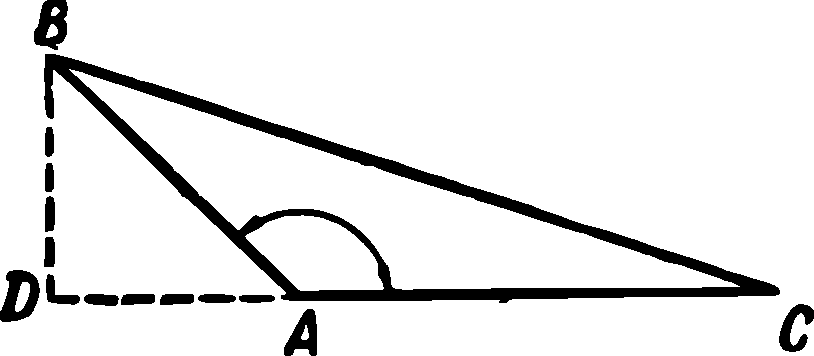
\includegraphics[width=0.8\textwidth]{figures/ch-05/fig-095.pdf}
\sidecaption{To the solution of the obtuse angle.\label{fig-095}}
\end{marginfigure}

It may happen that in the case of solving a triangle (on two sides and the angle between them), this angle is not sharp, but obtuse. If, for example, an obtuse angle $A$ and two sides, $AB$ and $AC$, are known in the ABC triangle (\figr{fig-095}), then the calculation of the remaining elements is as follows. Lowering the height $BD$, determine $BD$ and $AD$ from the triangle $BDA$; then, knowing $DA + AC$, find $BC$ and $\sin C$ by calculating the ratio $BD / BC$.


\section{Triangle Area Problem}
\label{sec-5.7}

\ques During an excursion, we measured the sides of a triangular area in steps and found them to be 43, 60, and 54 steps, respectively. What are the angles of this triangle?



\ans This is the most complex case of solving a triangle: by three sides. However, it can be managed without resorting to other functions besides sine. Dropping $BD$ (see \figr{fig-096}) the perpendicular from $B$ to the longest side $AC$, we have:
\begin{marginfigure}%[2cm]
\centering
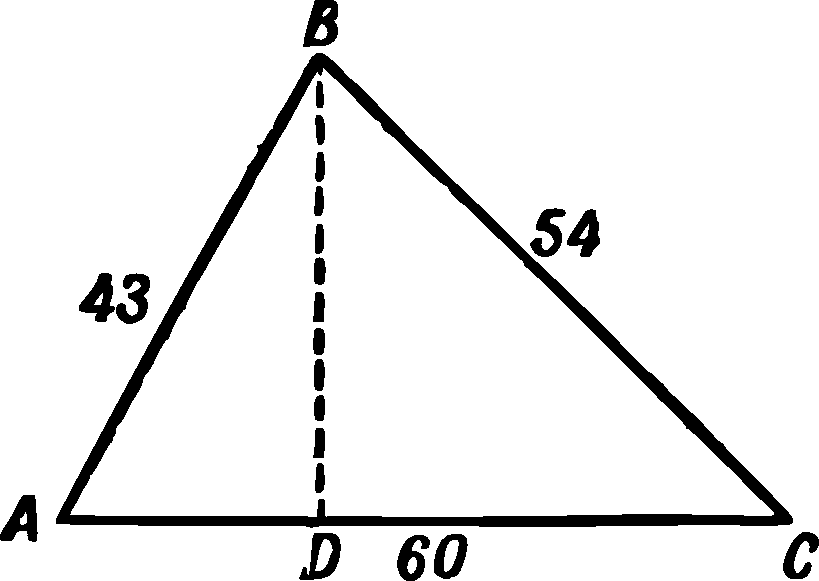
\includegraphics[width=\textwidth]{figures/ch-05/fig-096.pdf}
\sidecaption{Find the angles of this triangle 1) by calculation, 2) using a protractor.\label{fig-096}}
\end{marginfigure}
\begin{align*}%
BD^{2} & = 43^{2} - AD^{2}, \quad BD^{2} = 54^{2} - DC^{2},\,\, \text{hence}\\
43^{2} - AD^{2} & = 54^{2} - DC^{2},\\
DC^{2} - AD^{2} & = 54^{2} - 43^{2} = 1070.\\
\text{But} \,\,DC^{2} - AD^{2} & = (DC + AD)(DC - AD) = 60(DC - AD).  \\
\therefore \,\, 60(DC - AD) & = 1070 \qand DC - AD = 17.8. 
\end{align*}
From the equations $DC - AD = 17.8$ and $DC + AD = 60$, we get: 
$2DC = 77.8$, i.e. $DC = 38.9$. Now, it's easy to calculate the height:
\begin{equation*}%
BD = \sqrt{54^{2} - 38.9^{2}} = 37.4,
\end{equation*}
from which we find:
\begin{align*}%
\sin A & = \frac{BD}{AB} = \frac{37.4}{43} = 0.87; \quad A \approx \ang{60},\\
\sin C & = \frac{BD}{BC} = \frac{37.4}{54	} = 0.69; \quad A \approx \ang{44}.
\end{align*}
Then we can find angle $B = \ang{180} - (A + C) = \ang{76}$.

If we were to calculate this using tables, according to the rules of ``real'' trigonometry, we would get angles expressed in degrees and minutes. However, these minutes would be inherently erroneous, as the sides measured in steps involve an error of no less than 2–3\%. Hence, to avoid self-deception, the obtained ``accurate'' angle values should be rounded to at least whole degrees. And then we would arrive at the same result as we did by resorting to simplified methods. The benefit of our ``field'' trigonometry is quite evident here.


\section{Determining the Magnitude of an Angle without any Instruments}

To measure angles on the ground, we need at least a compass, and sometimes just our own fingers or a matchbox. But there may be a need to measure an angle drawn on paper, on a plan, or on a map.

Of course, if a protractor is at hand, the problem is easily solved. But what if there is no protractor, for example, in field conditions? A geometer should not be at a loss in this case either. How would you solve the following problem: 

\ques Angle $AOB$ (see \figr{fig-097}) is depicted, measuring \ang{180}. Determine its magnitude without measurements.
\begin{marginfigure}%[2cm]
\centering
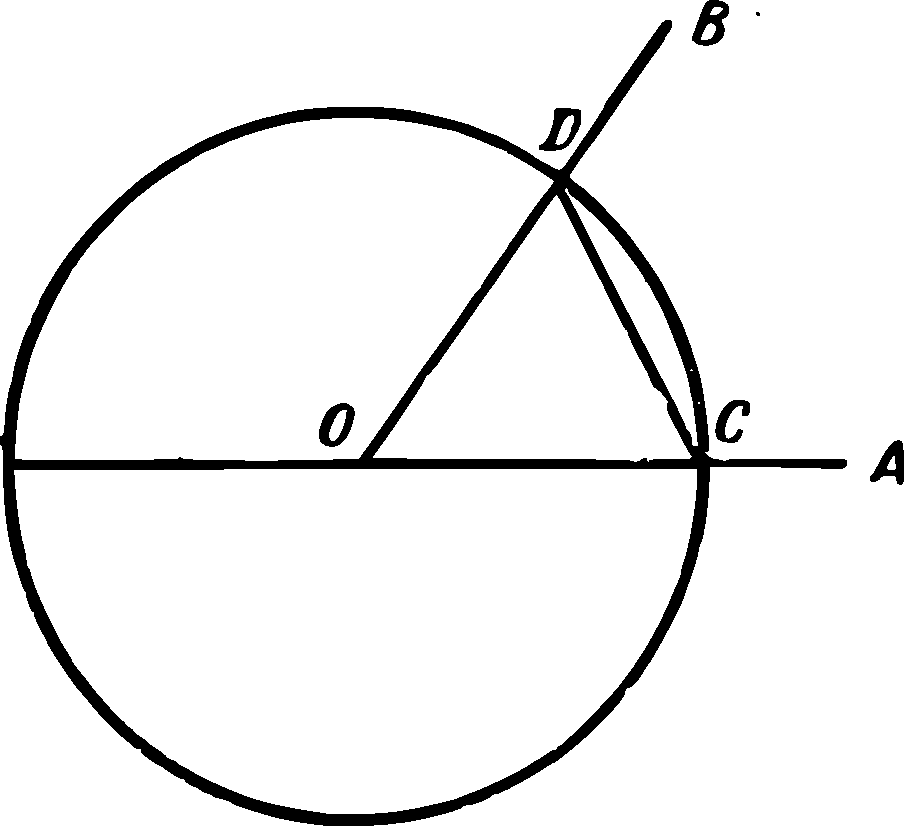
\includegraphics[width=\textwidth]{figures/ch-05/fig-097.pdf}
\sidecaption{97. How to determine the value of the depicted angle of the $AOB$ using only a compass?\label{fig-097}}
\end{marginfigure}

\ans One could drop a perpendicular from any point on side $BO$ to side $AO$, measure the catheti and the hypotenuse in the resulting right-angled triangle, find the sine of the angle, and then the magnitude of the angle itself (see page~\pageref{sec-5.3}). But such a solution would not meet the strict condition of not measuring anything!

Let's use the solution proposed in 1946 by J. Rupeika from Kaunas.

From vertex $O$, as from the centre, using the compass, let's draw a complete circle with any radius. Points $C$ and $D$, the intersections of the circle with the sides of the angle, are then connected by a straight line.

Now, using only the compass, starting from the initial point $C$ on the circle, we will sequentially lay off the chord $CD$ in the same direction until the compass leg coincides again with the starting point $C$.

While laying off the chords, we must count how many times the circle is circumvented during this time and how many times the chord is laid off.

Let's assume that we circled the circle $n$ times and during this time laid off the chord $CD$ $S$ times. Then the desired angle will be equal to 
\begin{equation*}%
\angle AOB = \frac{\ang{360}\cdot n}{S}.
\end{equation*}
Indeed, let the given angle contain \ang{x}; by laying off the chord $CD$ on the circle $S$ times, we, so to speak, increased the angle \ang{x} by $S$ times, but since the circle was circled $n$ times in the process, this angle will be $\ang{360} \times n$, i.e., $\ang{x} \cdot S = \ang{360} \cdot n; hence, 
\begin{equation*}%
\ang{x} = \frac{360° \cdot n}{S}.
\end{equation*}
For the angle depicted in the drawing, $n = 3$, $S = 20$ (check!); therefore, $ \angle AOB = \ang{54}$. In the absence of a compass, a circle can be drawn using a pin and a strip of paper; the chord can also be laid off using the same paper strip.

\ques Determine the angles of the triangle in \figr{fig-096} using this method.

\begin{center}
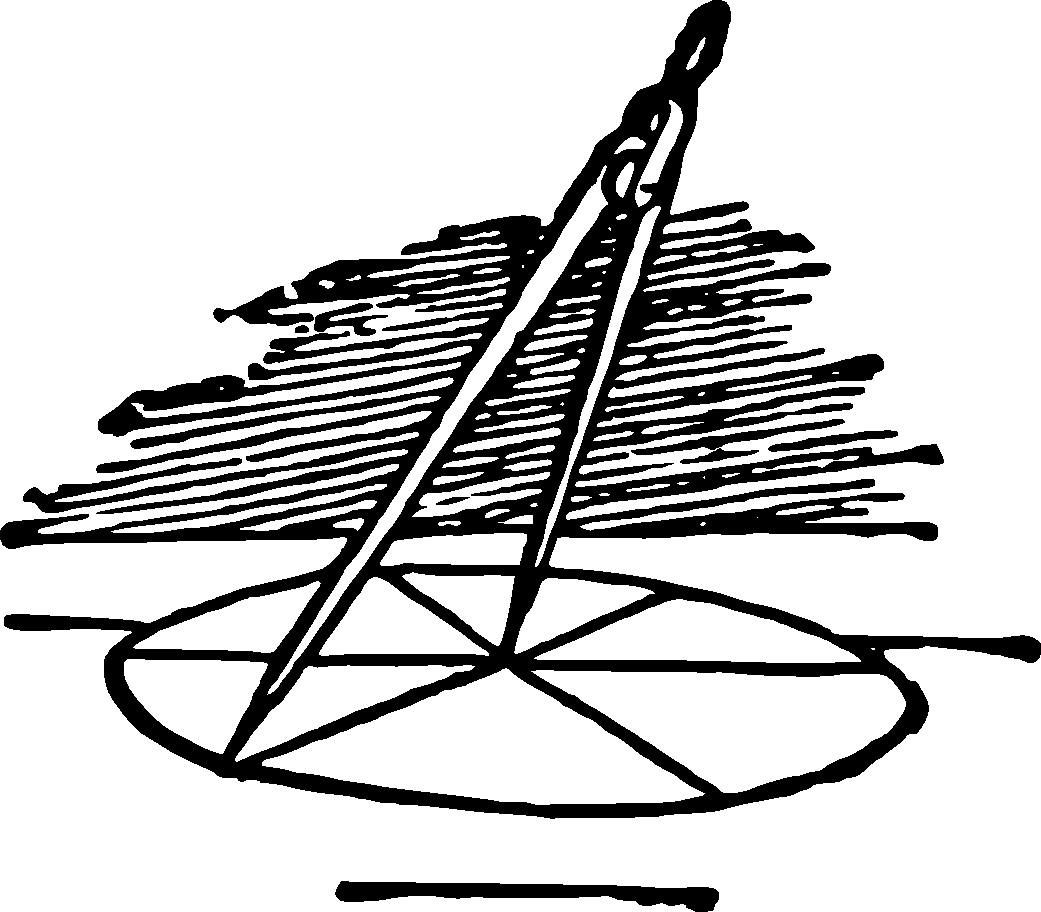
\includegraphics[width=0.3\textwidth]{figures/ch-05/fig-ch-05-tail.pdf}
\end{center}


















